\newpage
\section{Transformée de Fourier discrète}
Jusqu'à présent, les outils mathématiques exposés marchent bien, car on sait la forme exacte de la fonction d'intérêt. Cependant, lorsqu'on fait des expériences dans la vraie vie, il est impossible d'avoir autant d'informations. Par exemple, la prise de données ne peut se faire que de manière discrète.  Pour utiliser la TF dans ce contexte, ce qu'on nommera la transformée de Fourier discrète (TFD), il faudra la retravailler afin qu'elle utilise des données discrètes.

\subsection{Delta de Dirac et propriété d'échantillonnage}
Un delta de Dirac $\delta(x-x^*)$ est une "fonction" nulle partout sauf au point $x^*$ et dont $\int_{-\infty}^{\infty}\delta(x-x^*)dx = 1$. Par exemple, $\delta(x)$ est nulle partout sauf à l'origine. Naturellement, pour une fonction $f(x)$ quelconque, $f(x)\delta(x-x^*) = f(x^*)\delta(x-x^*)$. Dès lors, on remarque que 

\begin{equation*}
    \int_{-\infty}^{\infty}f(x)\delta(x-x^*)dx = \int_{-\infty}^{\infty}f(x^*)\delta(x-x^*)dx = f(x^*)\int_{-\infty}^{\infty}\delta(x-x^*)dx = f(x^*)  
\end{equation*}

Ainsi, depuis le delta de Dirac, on voit qu'il est possible d'échantillonner une valeur de $f(x)$ au point $x^*$. On peut répéter le processus pour différents points afin d'avoir un échantillonnage $\left\{f(x_k)\right\}_{k=0}^{N-1}$ de la fonction $f(x)$. Alors, on peut dire que

\begin{equation}
    f_{\text{éch.}}(x) = \sum_{k=0}^{N-1}f(x)\delta(x-x_k) = \sum_{k=0}^{N-1}f(x_k)\delta(x-x_k)
    \label{eq_fct_ech}
\end{equation}

où $f_{\text{éch.}}(x)$ est nulle sauf aux points échantillonnés. Autrement dit, (\ref{eq_fct_ech}) permet de modéliser ce qu'on aurait lors d'une prise de mesures. Cette propriété d'échantillonnage facilite grandement le passage de la TF à la TFD, bien qu'il y a beaucoup de subtilités en lien avec le delta de Dirac.

% \begin{figure}[H]
%     \centering
%         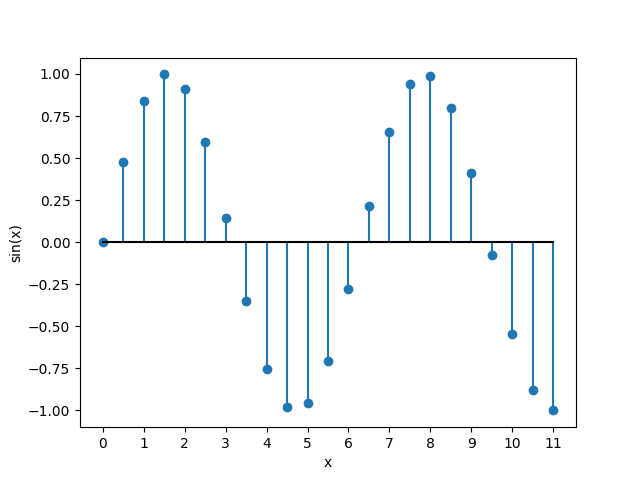
\includegraphics[width=0.48\textwidth]{images/ch4/echantillonage.png}
%     \caption{Exemple d'échantillonage de $\sin(x)$}
%     \label{fig_ech_sin}
%     \end{figure}

\subsection{Passage de la TF à la TFD}
Comme on l'a dit précédemment, dans la vraie vie, on enregistre une suite de $N$ points $\left\{f(t_k)\right\}_{k=0}^{N-1}$ à différents instants $t_k$. Par (\ref{eq_fct_ech}), on sait comment écrire la fonction échantillonnée. En la mettant dans (\ref{eq_TF}), on calcule 

\begin{equation*}
    c(\omega) = \int_{-\infty}^{\infty}f_{\text{éch.}}(t)e^{-i\omega t}dt = \int_{-\infty}^{\infty}\left(\sum_{k=0}^{N-1}f(t_k)\delta(t-t_k)\right)e^{-i\omega t}dt 
\end{equation*}
\begin{equation*}
    = \int_{-\infty}^{\infty}f(t_0)\delta(t-t_0)e^{-i\omega t_0}dt + \dots + \int_{-\infty}^{\infty}f(t_{N-1})\delta(t-t_{N-1})e^{-i\omega t_{N-1}}dt 
\end{equation*}
\begin{equation*}
    = f(t_0)e^{-i\omega t_0}\int_{-\infty}^{\infty}\delta(t-t_0)dt + \dots + f(t_{N-1})e^{-i\omega t_{N-1}}\int_{-\infty}^{\infty}\delta(t-t_{N-1})dt = \sum_{k=0}^{N-1}f(t_k)e^{-i\omega t_k}
\end{equation*}

Par la suite, on fait les hypothèses raisonnables qu'on commence les mesures au temps $t_0 = 0$ et que les points $f(t_k)$ sont pris à intervalles réguliers (disons après un temps $\tau$). Donc, on a une série de points $\left\{f(k\tau)\right\}_{k=0}^{N-1}$ et le calcul précédent devient

\begin{equation*}
    c(\omega) = \sum_{k=0}^{N-1}f(t_k)e^{-i\omega t_k} = \sum_{k=0}^{N-1}f(k\tau)e^{-i\omega k\tau}
\end{equation*}

Puis, il n'est pas vraiment nécessaire de regarder toutes les fréquences angulaires $\omega$. Par convivialité, comme on a $N$ échantillons, il serait pratique d'avoir $N$ fréquences angulaires à la sortie de la TFD. Pour y arriver, on peut faire comme si la suite de mesures étaient périodiques (ce que la fonction sous-jacente n'est pas nécessairement). Cela permet, à la même manière d'une série de Fourier, d'utiliser des fréquences angulaires discrètes. Ici, la période vaut $T = N\tau$, donc on remplace $\omega$ par $\frac{2\pi n}{T} = \frac{2\pi n}{N\tau}$ dans la dernière équation pour discrétiser la fréquence angulaire. On trouve 

\begin{equation}
    c_n = \sum_{k=0}^{N-1}f(k\tau)e^{-i\frac{2\pi n}{N\tau}k\tau} = \sum_{k=0}^{N-1}f_ke^{-i\frac{2\pi}{N}nk}
    \label{eq_TFD}
\end{equation}

Afin d'alléger l'écriture, on écrit que $f(k\tau) = f_k$ pour désigner le $k$ième point. Aussi, on note que $n$ est un entier se promenant entre 0 et $N-1$ par la périodicité de l'exponentielle complexe. Il y a donc $N$ fréquences angulaires en sortie comme on le souhaitait. Ainsi, (\ref{eq_TFD}) correspond la TFD et on isole un des $f_k$ pour obtenir la transformée de Fourier inverse discrète (TFID).

\begin{equation}
    \sum_{n=0}^{N-1}c_n e^{i\frac{2\pi}{N}nk^{'}} = \sum_{k=0}^{N-1}f_k\sum_{n=0}^{N-1} e^{-i\frac{2\pi}{N}n(k-k^{'})} = Nf_{k^{'}} \implies f_k = \frac{1}{N}\sum_{n=0}^{N-1}c_n e^{i\frac{2\pi}{N}nk}
    \label{eq_TFID}
\end{equation}

\subsection{Représentation matricielle}
Communément, il est pratique de compiler les $f_k$ et les $c_n$ dans des vecteurs.

\begin{equation*}
    \vec{f} = 
    \begin{bmatrix}
        f_0 \\
        \vdots \\
        f_{N-1} \\
    \end{bmatrix}, \ \
    \vec{c} = 
    \begin{bmatrix}
        c_0 \\
        \vdots \\
        c_{N-1} \\
    \end{bmatrix}
\end{equation*}

Avec cela, il est facile de déduire que la TFD correspond simplement à un produit matricielle entre une certaine matrice $U$ et le vecteur $\vec{f}$. En posant $W = e^{-i\frac{2\pi}{N}}$, il est facile de vérifier que 

\begin{equation*} 
    \begin{bmatrix}
        c_0 \\
        c_1 \\
        \vdots \\
        c_{N-1} \\
    \end{bmatrix}
    =
    \begin{bmatrix}
        1 & 1 & \dots & 1 & 1\\
        1 & W & \dots & W^{N-2} & W^{N-1}\\
        \vdots & \vdots & \ddots & \vdots & \vdots\\
        1 & W^{N-1} & \dots & W^{(N-1)(N-2)} & W^{(N-1)(N-1)}
    \end{bmatrix}
    \begin{bmatrix}
        f_0 \\
        f_1 \\
        \vdots \\
        f_{N-1} \\
    \end{bmatrix}
\end{equation*}

où $U = \left[W^{nk}\right]_{n,k=0}^{N-1}$. Pour faire la TFID, on a simplement à faire le produit entre $\frac{1}{N}$ fois le conjugué complexe de $U$ et le vecteur $\vec{c}$.

\begin{equation*} 
    \begin{bmatrix}
        f_0 \\
        f_1 \\
        \vdots \\
        f_{N-1} \\
    \end{bmatrix}
    = \frac{1}{N}
    \begin{bmatrix}
        1 & 1 & \dots & 1 & 1\\
        1 & W & \dots & W^{N-2} & W^{N-1}\\
        \vdots & \vdots & \ddots & \vdots & \vdots\\
        1 & W^{N-1} & \dots & W^{(N-1)(N-2)} & W^{(N-1)(N-1)}
    \end{bmatrix}^*
    \begin{bmatrix}
        c_0 \\
        c_1 \\
        \vdots \\
        c_{N-1} \\
    \end{bmatrix}
\end{equation*}

Grâce à la représentation matricielle, on voit qu'il y a un total de $N (N-1)$ additions/soustractions complexes à faire ainsi que $N^2$ multiplications complexes à réaliser autaut pour calculer la TFD que la TFID. En effet, il y a $N$ éléments à calculer demandant chacun $N$ multiplications complexes et $N-1$ additions/soustractions complexes. 
